The signals we obtained from the experiment were analyzed and interpreted using the methods presented in this chapter. Starting with specifics of the data collection process, we continue by discussing signal processing algorithms and feature extraction, and end with details on classification procedure.

\section{Data Collection}
As mentioned in section \ref{physmeas}, the psychophysiological measures, selected for this thesis, were blood volume pulse (\gls{bvp}), galvanic skin response (\gls{gsr}), and skin temperature. These signals were recorded using the integrated Photoplethysmography (\gls{ppg}), Electrodermal Activity (EDA), and Infrared Thermopile sensors of the Empatica E4 wristband. All recordings were conducted using a sampling frequency of 64Hz for \gls{bvp}, and 4Hz for both \gls{gsr}, and skin temperature. 
From the 14 subjects that partook in our experiment we obtained 14 sets of physiological data. The data of one subject was removed due to substantial artifact contamination, resulting in a total of 13 sets of physiological data that were used in the subsequent process. Each set was comprised of roughly 80-90 minutes of recordings, which complied to approximately 326.400 samples for \gls{bvp}, and 20.400 samples for \gls{gsr}, and skin temperature. 
The collected data was continuously streamed to a TCP client, running on the nearby Processing Unit, via a Bluetooth connection and saved into csv files after every full minute of recording. The saved files contained data samples of all three data streams and were named following the pattern shown in \ref{recpattern}.
\begin{equation} \label{recpattern}
\text{recording\_yyyy-mm-dd-hh-mm-ss}
\end{equation}
Then again, each data sample was comprised of three components which identified the data stream, the sample time, and the sample value. An example of this pattern is shown in \ref{samplepattern} for a sample of the BVP signal stream. 
\begin{equation}\label{samplepattern}
\text{E4\_Bvp 1569592961,01857 25,33795}
\end{equation}

\section{Data Preparation}
As the data was saved in a number of individual csv files the goal of the initial step of data processing was dedicated to translate the data samples into a usable format and separate the individual data stream (i.e. BVP, GSR, and skin temperature). This goal was achieved using two simple python scripts. The first program would locate all csv files in a certain folder and seamlessly merge them to a single csv file. Afterwards, the second script was used to scan all entries of this new file and sort them by their stream tag, which was indicated by the first portion of each data sample (see \ref{samplepattern}), using a simple string comparison method. This process resulted in a total of 6 data files (i.e. 2 files per data stream), of which each file contained either the sample values or the sample times of a single data stream. This format made the data easily distinguishable and accessible for the final step of data preparation, which was data segmentation. We divided the data streams into segments that were associated with the individual sessions of the experiment, using automatic timestamps that were generated during the experiment. The extracted segments were then saved in individual files that were appropriately named to provide explicit information about their content to facilitate subsequent processing steps. The naming pattern is shown in \ref{segmentpattern}.
\begin{equation}\label{segmentpattern}
\text{\_DataStream\_Datatype\_SubjectID\_SessionLabel\_StartTime\_EndTime}
\end{equation}

\section{Data Analysis}
All aspects of data analysis were handled using the programming language Python in combination with the PyCharm IDE. Therefore, this section is dedicated to explaining the general strategy, as well as the scripts that were built in the process of managing data processing, and feature extraction tasks.

\subsection{BVP}
\subsubsection{Pre-Processing}
% 	- PEAK DETECTION
%		- bandpass zero phase filtering
%		- clipping
%		- squaring
%		- moving averages
%		- thresholding
%		- blocks of interest
%		- peak detection
%		- peak validation
The main objective of BVP pre-processing was the detection of AC pulses, or $\alpha$ waves, in the BVP signal. To guarantee high quality peak detection even under challenging conditions, we implemented an algorithm that was introduced by Elgendi et al. (2013) for this very reason. The peak detection algorithm is based on event-related moving averages with dynamic thresholds, and is comprised of three main stages: pre-processing (bandpass filtering and squaring), feature extraction (generating potential blocks using two moving averages), and classification (thresholding)\cite{Elgendi2013}. 

%[insert: bvp_dt.jpg, source: \cite{Elgendi2013}]
%\begin{figure}[ht]
%	\centering
%  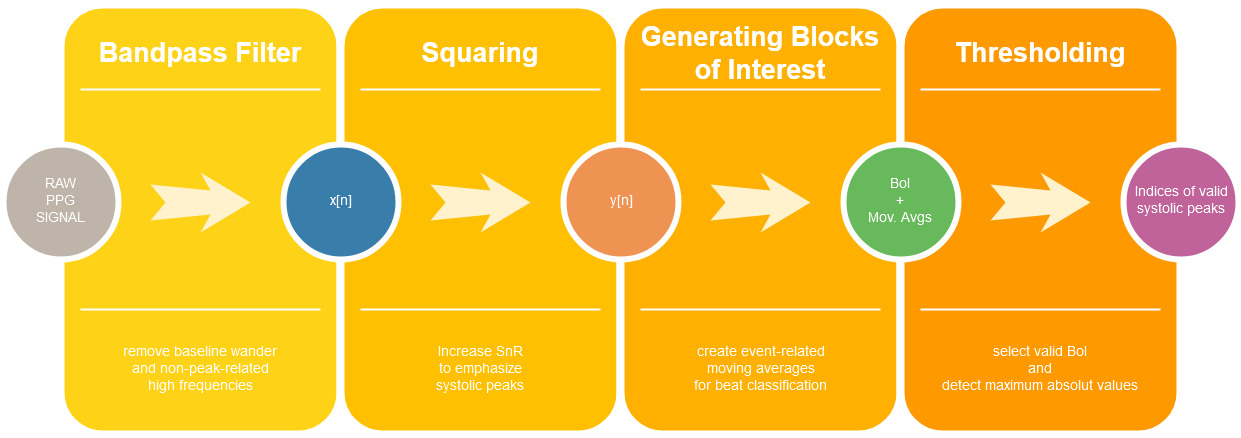
\includegraphics[width=1.0\textwidth, angle=0]{images/bvp_dt.jpg}
%	\caption[Peak Detection Algorithm]{Peak Detection Algorithm by Elgendi et al. (2013). This systolic peak time-domain detection algorithm consists of three main stages: pre-processing (bandpass filter, squaring), feature extraction (two moving averages), and classification (thresholding).}
%	\label{bvp_dt}
%\end{figure}

%The general structure of the algorithm is shown in \ref{bvp_dt}. 
The following paragraph will elaborate on the individual steps of the algorithm.\\
\textbf{Bandpass Filtering.} A zero-phase second-order Butterworth filter, with a bandpass of 0.5-8 Hz was implemented to remove baseline wander and non-peak-related high frequency components. The filter output was then applied to the raw PPG signal resulting in the filtered signal $S[n]$.\\
\textbf{Clipping.} In preparation of the next step of the algorithm, the filtered signal was clipped by removing the signal below zero. This resulted in the clipped signal $Z[n]$.\\
\textbf{Squaring.} Squaring was used to emphasize large differences resulting from the systolic waves, while simultaneously suppressing smaller differences caused by diastolic waves and noise \cite{Elgendi2013}.
This resulted in the signal $y[n]$ which is equal to $Z[n]^{2}$\\
\textbf{Generating Blocks of Interest.} Blocks of interest are generated using the two event-related moving averages $MA_{peak}$ and $MA_{beat}$. $MA_{peak}$ was used to mark systolic peak areas in $y[n]$ and is given by the equation \ref{ma_peak}. Where $W_{1}$ represented the window size of the systolic peak duration and was set to a value of 111 ms.\\
\begin{equation}\label{ma_peak}
MA_{peak}[n] = \frac{1}{W_{1}}\cdot(y[n-\frac{W_{1}-1}{2}]+...+y[n]+...+y[n+\frac{W_{1}-1}{2}])
\end{equation}
$MA_{beat}$ was used to mark heartbeat areas and given by the equation \ref{ma_beat}. Where $W_{2}$ represented the window size of one heartbeat duration and was set to a value of 667 ms.\\
\begin{equation}\label{ma_beat}
MA_{beat}[n] = \frac{1}{W_{2}}\cdot(y[n-\frac{W_{2}-1}{2}]+...+y[n]+...+y[n+\frac{W_{2}-1}{2}])
\end{equation}
\textbf{Thresholding.} The first dynamic threshold $THR_{1}$ was used to mark potential peak areas in $y[n]$ by creating a block of interest for every interval where $THR_{1}$ was greater than $MA_{peak}$. $THR_{1}$ was derived from $MA_{beat}$ following equation \ref{thr1}.
\begin{align} \label{thr1}
THR_{1} &= MA_{beat}[n]+\alpha \\
\alpha &= \beta\cdot\overline{z}
\end{align}
\newpage
Where $\beta$ was set to a constant value of 0,02 and $\overline{z}$ was the statistical mean of $y[n]$. Figure \ref{bvp_dta} demonstrates the idea of using two moving averages to generate blocks of interest.

%[insert: bvp_dta.jpg, source: \cite{Elgendi2013}]
\begin{figure}[h!]
	\centering
  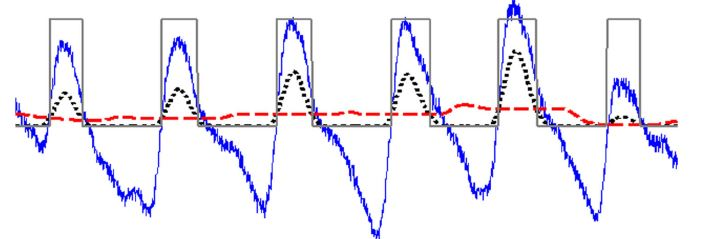
\includegraphics[width=1.0\textwidth, angle=0]{images/bvp_dta.jpg}
	\caption[Peak Detection Algorithm]{Blocks of interest are shown as grey squares over the filtered signal (in blue). The blocks are generated, using the two moving averages $MA_{peak}$ and $MA_{beat}$, which are depicted as a black dotted signal and a dashed red signal respectively. (source: doi:10.1371/journal.pone.0076585.g009)}
	\label{bvp_dta}
\end{figure}

Although this process generated many blocks, only some of them would contain the desired feature (i.e. the systolic peak). Therefore, it was necessary to identify and reject the blocks that resulted from diastolic waves and noise. The rejection was based on the second threshold $THR_{2}$, which corresponded to the anticipated width of a systolic peak and was set to $W_{1}$. Whenever a block was wider than or equal to $THR_{2}$ it was classified as valid.\\
\textbf{Peak Detection.}\label{pkdet} In the last step of the algorithm systolic peaks were detected by localizing the maximum absolute value in valid blocks of interest. 

\subsubsection{Inter-Beat-Intervals}
Using the indices of valid systolic peaks that were detected in \ref{pkdet}, the Inter-beat-interval tachogram was calculated as follows.
\begin{equation}
IBI_{i} = R_{i}-R_{i-1}
\end{equation}
Where Peaks are symbolically labeled $R$ to express their correspondence to the R-waves of the ECG, which are commonly used to calculate IBIs, and $i$ is the index value of the peak series.
Initially calculated in samples, the IBIs were then translated into milliseconds.

\subsubsection{Data Correction}
This section is dedicated to the treatment of ectopic beats, arrhythmic events, missing data, and artifacts in the IBI series. \\
\textbf{Outlier Rejection.} All IBIs that were considered physiologically impossible were marked as outliers. We used the HR-related thresholds $HR_{max}$ and $HR_{min}$ to calculate the shortest ($IBI_{min}$) and the longest ($IBI_{max}$) acceptable interval duration. $HR_{max}$ was determined using \ref{hrmax} and $HR_{min}$ was set to 45 beats per minute.
\begin{align}\label{hrmax}
HR_{max} &= \text{Maximum Physiological HR} - \text{Average Subject Age}\\
IBI_{min} &= \frac{60000}{HR_{max}}	[ms]\\
IBI_{max} &= \frac{60000}{HR_{min}}	[ms]
\end{align}
The resulting values for the new IBI-related thresholds $IBI_{max}$ and $IBI_{min}$ were rounded to the next full integer and then used to identify outliers in the IBI series. Afterwards, all marked IBI were replaced using linear interpolation.\\
\textbf{Ectopic Beat Identification.} To identify IBIs that resulted from ectopic beats we considered Kamath's suggestion. Thereby, a heartbeat interval was considered abnormal when the heartbeat interval increased by more than 32.5\% decreased by more than 24.5\% compared to the previous heartbeat \cite{Choi2016}. Equation \ref{kamath} shows the mathematical expression that was used as thresholding method for ectopic beat identification. 
\begin{equation} \label{kamath}
IBI_{EB} = \lbrace IBI\vert 0.675 IBI_{n-1} < IBI_{n} < 1.245 IBI_{n-1}\rbrace  
\end{equation}
\textbf{Artifact Rejection.} To increase the robustness of the HRV analysis all regions with the presence of ectopic beats or noise for more than 3 seconds were removed entirely \cite{Clifford2002}.\\
\textbf{Linear Interpolation.} We used linear interpolation to replace outliers and ectopic beats. First, IBIs immediately preceding and after the ectopic beat were marked for replacement. Afterwards, the total time encompassed by all marked IBIs was determined and the number of new beats $B$, that were inserted to replace them, was computed equation \ref{Bsingle} for single ectopic beats and equation \ref{Bseq} for a sequence of ectopic beats.
\begin{equation}\label{Bsingle}
B = \frac{IBI_{i}+IBI_{i+1}}{(IBI_{i-1}+IBI_{i+2})/2}
\end{equation}
\begin{equation}\label{Bseq}
B = \frac{\sum_{j=i}^{i+N} IBI_{i}}{(IBI_{i-1}+IBI_{i+N+1})/2}
\end{equation}
As $B$ would in general not be an integer value, the computed values were rounded to obtain the nearest integer. After the determination of the number of IBIs to insert was completed, the values of said IBIs were computed using linear interpolation. The basic principle is shown in figure \ref{ebrep}.

%[insert: bvp_dt.jpg, source: \cite{Lippman1994}]
\begin{figure}[h!]
	\centering
  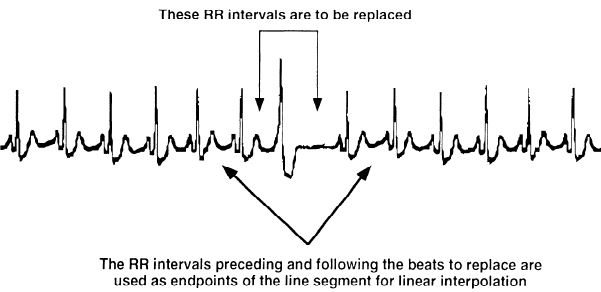
\includegraphics[width=1.0\textwidth, angle=0]{images/eb_replacement.jpg}
	\caption[Linear Interpolation of Ectopic Beats]{A schematic of linear interpolation of ectopic beats on an ECG signal. RR-intervals before and after the ectopic beat are marked for replacement (vertival arrows). RR-intervals before and after the marked segment are used for interpolation (diagonal arrows). source: \cite{Lippman1994}}
	\label{ebrep}
\end{figure}
\textbf{Data Rejection.} For short term recordings, such as the ones we conducted in this thesis, it is recommended that at least 80\% of a 5 minute segment of data should contain acceptable IBIs \cite{Clifford2002}. Therefore, recordings that failed this condition were barred from the subsequent feature extraction.

% INTER BEAT INTERVALS
%	- DETECT OUTLIER
%	- DETECT ECTOPIC BEATS
%	- ARTIFACT DECLARATION
%	- LINEAR INTERPOLATION
%DATA VALIDATION

\newpage
\subsubsection{Feature Extraction}
 %FEATURE EXTRACTION
HRV feature extraction was based entirely on the recommendations given by the Task Force (1996). The selected measures are shown in the tables below, sorted by their domains.

\begin{table}[h!]
\caption[HRV Feature Selection 1]{HRV Feature Selection 1}
\begin{tabular}{cccc}
\multicolumn{4}{c}{\thead{Time Domain Measures}} \\
\hline 
\thead{Variable} & \thead{Units} & \thead{Description} & \\ 
\multicolumn{4}{c}{Statistical Measures} \\ 
 & & & \\
\hline
 & & & \\
SDNN & $ms$ & \multicolumn{2}{c}{\makecell[l]{Standard deviation of all inter beat  intervals}} \\ 
RMSSD & $ms$ & \multicolumn{2}{c}{\makecell[l]{The square root of the mean of the sum of the squares \\ of differences between adjacent inter beat intervals}} \\ 
SDSD & $ms$ & \multicolumn{2}{c}{\makecell[l]{Standard deviation of differences between adjacent \\ inter beat intervals}} \\ 
IBI50 &  & \multicolumn{2}{c}{\makecell[l]{Number of pairs of adjacent inter beat intervals \\ differing by more than 50 ms in the entire recording}} \\ 
pIBI50 & $\%$ & \multicolumn{2}{c}{\makecell[l]{IBI50 divided by the total number of all inter beat intervals}} \\ 
mIBI & $ms$ & \multicolumn{2}{c}{\makecell[l]{Mean of all inter beat intervals}} \\
mHR & $bpm$ & \multicolumn{2}{c}{ \makecell[l]{Mean heart rate of the entire recording}}\\
rIBI & $ms$ & \multicolumn{2}{c}{\makecell[l]{The difference between the longest and the shortest \\ inter beat interval}}\\
& & & \\
\hline
\end{tabular} 
\end{table}

\begin{table}[h!]
\caption[HRV Feature Selection 2]{HRV Feature Selection 2}
\begin{tabular}{cccc}
\multicolumn{4}{c}{\thead{Frequency Domain Measures}} \\
\hline 
\thead{Variable} & \thead{Units} & \thead{Description} & \thead{Frequency range}\\ 
\multicolumn{4}{c}{Analysis of short-term recordings (5min)} \\ 
 & & & \\
\hline
 & & & \\
Total power & $ms^2$ & \makecell[l]{The variance of all \gls{ibi}} & $\leq$ 0.4 Hz\\
VLF & $ms^2$ & \makecell[l]{Power in very low frequency range} & $\leq$ 0.04 Hz\\
LF & $ms^2$ & \makecell[l]{Power in low frequency range} & 0.04-0.15 Hz\\
nLF & $n.u.$ & \makecell[l]{LF power in normalized units \\ LF/(Total Power–VLF)$\cdot$100} & \\
HF & $ms^2$ & \makecell[l]{Power in high frequency range} & 0.15-0.4 Hz\\
nHF & $n.u.$ & \makecell[l]{HF power in normalized units \\ HF/(Total Power–VLF)$\cdot$100} & \\
LF/HF &  & \makecell[l]{Ratio of LF power to HF power} & \\
& & & \\
\hline
\end{tabular} \label{freqfeat}
\end{table}

The power for the three spectral components (see \ref{freqfeat}) is represented by the average bandpower in the respective frequency range. In order to calculate the average bandpower, we used Welch's method in conjunction with a Hann window. Which is a commonly used method to compute an estimate of the spectral density by dividing the data into overlapping segments, computing a modified periodogram for each segment, and averaging the periodograms. Afterwards, the resulting frequency bins were assigned to the respective bands and the absolute power was approximated by integration ,using the composite trapezoidal rule. The data that was subjected to spectral analysis was obtained by creating a discrete event series, using the \gls{ibi} tachogram, and interpolating it with a sampling frequency of 7 Hz. 


\newpage

\subsection{GSR}
\subsubsection{Pre-Processing}\label{gsrpp}
% GSR PRE PROCESSING
%	- low pass zero phase filtering
%	- smoothing: moving average filtering
As we were only interested in the tonic component of GSR, pre-processing was focused primarily on artifact removal and noise reduction. The following paragraph covers all measures that were applied in the process of pre-processing.\\
\textbf{Lowpass Filtering.} A zero-phase fourth-order Butterworth lowpass filter, with a cutoff frequency of 1.0 Hz was implemented to remove high frequency artifacts, caused by electrode movement or electrical noise.\\
\textbf{Mean Correction.} To account for environmental influences such as temperature and humidity the filtered signal was corrected using the mean GSR value of the baseline measurement. The mean corrected data was then subjected to the feature extraction methods.
\subsubsection{Feature Extraction}\label{gsrfe}
% FEATURE EXTRACTION
GSR feature extraction was focused on deriving a number of basic statistical time domain measures. The selected measures are shown in the table below.
\begin{table}[h!]
\caption[GSR Feature Selection]{GSR Feature Selection}
\begin{tabular}{cccc}
\multicolumn{4}{c}{\thead{Time Domain Measures}} \\
\hline 
\thead{Variable} & \thead{Units} & \thead{Description} & \\ 
\multicolumn{4}{c}{Statistical Measures} \\ 
 & & & \\
\hline
 & & & \\
mGSR & $\mu S$ & \multicolumn{2}{c}{\makecell[l]{Mean value of the entire recording}} \\ 
rGSR & $\mu S$ & \multicolumn{2}{c}{\makecell[l]{The difference between the lowest and the highest value}} \\
sdGSR & $\mu S$ & \multicolumn{2}{c}{\makecell[l]{The standard deviation of the entire recording}} \\
& & & \\
\hline
\end{tabular} 
\end{table}

\newpage
\subsection{Skin Temperature}
\subsubsection{Pre-Processing}
% TEMPERATURE PRE PROCESSING
%	- smoothing: moving average filtering
The pre-processing of the skin temperature signal was identical to the methods applied to the GSR signal. Therefore, we refer to section \ref{gsrpp} at this point.
\subsubsection{Feature Extraction}
% FEATURE EXTRACTION
Similar to \ref{gsrfe}, feature extraction was focused on deriving a number of basic statistical time domain measures. The selected measures are shown in the table below.
\begin{table}[h!]
\caption[Skin Temperature Feature Selection]{Skin Temperature Feature Selection}
\begin{tabular}{cccc}
\multicolumn{4}{c}{\thead{Time Domain Measures}} \\
\hline 
\thead{Variable} & \thead{Units} & \thead{Description} & \\ 
\multicolumn{4}{c}{Statistical Measures} \\ 
 & & & \\
\hline
 & & & \\
mST & $^{\circ}C$ & \multicolumn{2}{c}{\makecell[l]{Mean temperature of the entire recording}} \\ 
rST & $^{\circ}C$ & \multicolumn{2}{c}{\makecell[l]{The difference between the lowest and the highest value}} \\
sdST & $^{\circ}C$ & \multicolumn{2}{c}{\makecell[l]{The standard deviation of the entire recording}} \\
& & & \\
\hline
\end{tabular} 
\end{table}

\newpage
\section{Data Interpretation}\label{datainterpretation}
% ml methods
Similar to data analysis, we handled data interpretation using the programming language Python in combination with the PyCharm IDE. In particular, we used the scikit-learn package to implement data and feature preparation methods, as well as parameter optimization in the training process.

\subsection{Preparation} 
\textbf{Formatting.} During the feature extraction process, extracted features from one session were separated by signal type and stored in individual Python dictionaries. Therefore, a subroutine was built to extract the features from their individual dictionaries and sort them by the session they originated from. The resulting data points were comprised of all features that were extracted from one recording session (e.g. a 5 minute baseline recording).
Afterwards, those data points were converted into a NumPy array with the dimensions $n \times f$, where $n$ was the number of data points (i.e. the sum of all recorded sessions of all the subjects) and $f$ was the number of features that were extracted for each data point.\\
\textbf{Generating Training and Test Sets.} A common practice in machine learning to prevent a classifier from overfitting is to reserve some of the data for testing and validation purposes. Therefore, the data set was divided into training and test samples. Approximately 25\% of data points were reserved for algorithm testing, and the remaining 75\% were used for training purposes. This step was implemented using the $\text{\_train\_test\_split}$ helper function in the scikit-learn toolbox.\\
\textbf{K-fold Crossvalidation} is a convenient way to facilitate the evaluation of the training process without having to resort to the test samples. By employing k-fold Crossvalidation on the training set we were able to compensate for the small sample size of our data set while still reserving the test samples for the final validation.\\
\textbf{Feature Preparation.} The performance of some machine learning techniques is extremely dependent on data representation. In particular, SVM and Neural Networks benefit from data Normalization (i.e. features are represented as values between 0 and 1). Therefore, we used Python's $\text{MinMaxScaler}$ function to translate each feature individually to a range of 0 to 1.\\

\newpage
\subsection{Data Sets} 
A number of subsets were created to explore classification accuracy for a variety of different scenarios. Therefore, data points were sorted by their session type and recombined to build the subsets shown in \ref{MLDS}.
\begin{table}[h!]
\caption[Machine Learning Data Sets]{Machine Learning Data Sets}
\begin{flushleft}
\begin{tabular}{cccc}
\hline 
\thead{\makecell[c]{Set Name}} & \thead{Description} & & \thead{\makecell[c]{Targets}}\\ 
\multicolumn{4}{c}{Complete Sets } \\ 
 & & & \\
\hline
 & & & \\
Original & \multicolumn{2}{c}{\makecell[l]{The set contains all recording sessions. \\ Each session type has an individual label.}} & 6 \\
Rest Vs All & \multicolumn{2}{c}{\makecell[l]{The set contains all recording sessions. \\ All session types, except for the baseline sessions, \\ have the same label.}} & 2 \\ 
Stress Vs All & \multicolumn{2}{c}{\makecell[l]{The set contains all recording sessions. \\ All session types, except for the stress sessions, \\ have the same label.}} & 2 \\ 
Emotion Vs All & \multicolumn{2}{c}{\makecell[l]{The set contains all recording sessions. \\ All session types, except for the visual \\ stimulation sessions, have the same label.}} & 2 \\ 
 & & & \\
\multicolumn{4}{c}{Reduced Sets} \\ 
 & & & \\
\hline
 & & & \\
Stress Vs Rest & \multicolumn{2}{c}{\makecell[l]{The set contains only stress and baseline sessions. \\ Each session type has an individual label.}} & 2 \\
Stress Vs Stress & \multicolumn{2}{c}{\makecell[l]{The set contains only stress sessions. \\ Each session type has an individual label.}} & 2 \\
Emotion Vs Emotion & \multicolumn{2}{c}{\makecell[l]{The set contains only visual stimulation sessions. \\ Each session type has an individual label.}} & 2 \\
& & & \\
\hline
\end{tabular} \label{MLDS}
\end{flushleft}
\end{table}

\subsection{Feature Sets} 
Optimizing feature selection is a key component for the success of machine learning. Therefore, a number of feature sets were created to explore the effects on the classification accuracy of the chosen machine learning algorithms. The individual sets are listed below.
\begin{itemize}
\item \textbf{Original:} This set was comprised of 21 features from all three physiological signals. Including time domain methods of HRV, GSR, and skin temperature, as well as HRV frequency domain methods.
\item \textbf{Reduced T:} This set was comprised of 14 features of all three physiological signals. Including only time domain methods of HRV, GSR, and skin temperature.
\item \textbf{Reduced F:} This set was comprised of 13 features of all three physiological signals. Including only HRV frequency methods, as well as time domain methods of GSR, and skin temperature.
\item \textbf{Single Sets:} These sets were only comprised of a certain feature group of one physiological measures. Resulting in a set for each of the following: HRV time measures (8 features), HRV frequency measures (7 features), GSR time measures (3 features), and skin temperature time methods (3 features).
\end{itemize}

\subsection{Data Classification}
As described in section \ref{mlsel}, we selected the following four machine learning algorithms for classification.
\begin{enumerate}
\item \textbf{k-NN Classifier}
\item \textbf{Random Forest Classifier}
\item \textbf{Support Vector Machines}
\item \textbf{Neural Networks}
\end{enumerate}

After coding subroutines for each of the above, using their respective implementations in scikit-learn we conducted a Gridsearch for algorithm specific hyper-parameters with the goal of performance optimization. Hyper-parameters are parameters that are not directly learned within estimators. In scikit-learn they are passed as arguments to the constructor of the estimator classes (e.g. C, kernel and gamma for SVM).
The Gridsearch was managed using the $\text{GridSearchCV}$ method, which exhaustively generates candidates from a grid of parameter values ($\text{param\_grid}$). Tables \ref{paramgrids1} and \ref{paramgrids2} show the parameter grids that were employed in this process. Also, k-fold Crossvalidation (k=3, 5) was applied in the process.
\begin{table}[h!]
\caption[Gridsearch Parameters Part 1]{Gridsearch Parameters Part 1}
\begin{flushleft}
\begin{tabular}{cccc}
\hline 
\thead{\makecell[c]{Parameter}} & \thead{Description} & & \thead{\makecell[c]{Values}}\\ 
\multicolumn{4}{c}{\textbf{k-NN Classifier}} \\ 
 & & & \\
\hline
 & & & \\
$\text{n\_neighbors}$ & \multicolumn{2}{c}{\makecell[l]{The number of neighbors that is considered.}} & 1-12 \\
 & & & \\
\multicolumn{4}{c}{\textbf{Support Vector Classifier}} \\ 
 & & & \\
\hline
 & & & \\
$\text{kernel}$ & \multicolumn{2}{c}{\makecell[l]{Specifies the kernel type to be \\used in the algorithm.}} & rbf \\
$\text{C}$ & \multicolumn{2}{c}{\makecell[l]{Regularization parameter. The \\strength of the regularization is \\ inversely proportional to C. }} & \makecell[c]{0.001, 0.01, 0.1, 1,\\ 10, 100, 150, 200} \\
$\text{gamma}$ & \multicolumn{2}{c}{\makecell[l]{The kernel coefficient. }} & \makecell[c]{0.0001, 0.001, 0.01, 0.1,\\ 1, 10, 50, 100}\\
 & & & \\
\hline
\end{tabular} \label{paramgrids1}
\end{flushleft}
\end{table}

\begin{table}[h!]
\caption[Gridsearch Parameters Part 2]{Gridsearch Parameters Part 2}
\begin{flushleft}
\begin{tabular}{cccc}
\hline 
\thead{\makecell[c]{Parameter}} & \thead{Description} & & \thead{\makecell[c]{Values}}\\ 
\multicolumn{4}{c}{\textbf{Random Forest Classifier}} \\ 
 & & & \\
\hline
 & & & \\
$\text{n\_estimators}$ & \multicolumn{2}{c}{\makecell[l]{The number of trees in the forest}} &  \makecell[c]{5, 25, 50, 100,\\ 250, 500, 1000}\\
$\text{max\_depth}$ & \multicolumn{2}{c}{\makecell[l]{The maximum depth of the tree.}} &  \makecell[c]{1-5}\\
$\text{max\_features}$ & \multicolumn{2}{c}{\makecell[l]{The number of features to consider \\when looking for the best split. Because we\\ use float values int($\text{max\_features} \cdot \text{n\_features}$)\\ features are considered at each split.}} &  \makecell[c]{0.10, 0.25, 0.5,\\ 0.75, 1.0}\\
 & & & \\
\multicolumn{4}{c}{\textbf{Neural Networks}} \\ 
 & & & \\
\hline
 & & & \\
$\text{solver}$ & \multicolumn{2}{c}{\makecell[l]{The solver for weight optimization.}} &  \makecell[c]{lbfgs}\\
$\text{activation}$ & \multicolumn{2}{c}{\makecell[l]{The activation function for the\\ hidden layer.}} &  \makecell[c]{tanh, relu}\\
$\text{hidden\_layer\_size}$ & \multicolumn{2}{c}{\makecell[l]{The number of neurons in each layer. \\We used 1-3 layers, with identical\\ amounts of neurons, determined by \\int($\text{max\_features} \cdot \text{hidden\_layer\_size}$).}} &  \makecell[c]{0.5, 1, 2}\\
$\text{alpha}$ & \multicolumn{2}{c}{\makecell[l]{L2 penalty (regularization term)\\ parameter.}} &  \makecell[c]{0.00001, 0.0001,\\ 0.0005, 0.001, 0.005, \\0.01, 0.05, 0.1, 0.5, 1}\\
$\text{learning\_rate}$ & \multicolumn{2}{c}{\makecell[l]{The learning rate is used to control the \\step-size in updating the weights.}} &  \makecell[c]{0.001, 0.01, 0.1}\\
 & & & \\
\hline
\end{tabular} \label{paramgrids2}
\end{flushleft}
\end{table}
Afterwards, the best estimators for each feature- and data set combination were determined by comparing Crossvalidation scores. Lastly, the final validation was conducted using the best estimators on the reserved test data sets.
